\documentclass[11pt,a4paper]{article}
\usepackage[T1]{fontenc}
\usepackage[ngerman]{babel}
\usepackage{amsmath}
\usepackage{parskip}
\usepackage{graphicx}
\usepackage{listings}

%opening
\author{Simon Cholewa}
\title{2. Excercises MAT}

\hyphenation{
	Mo-tor-ü-ber-wach-ung 
}


\begin{document}

\maketitle

\section{IDE Set Up}
\textit{A1: Set up a sound development environment. Minimum is Sublime Text.}

Abbildung \ref{fig:pycharm} auf zeigt einen Screenshot meiner PyCharm-Installation.

\begin{figure}[!htbp] 
	\centering
	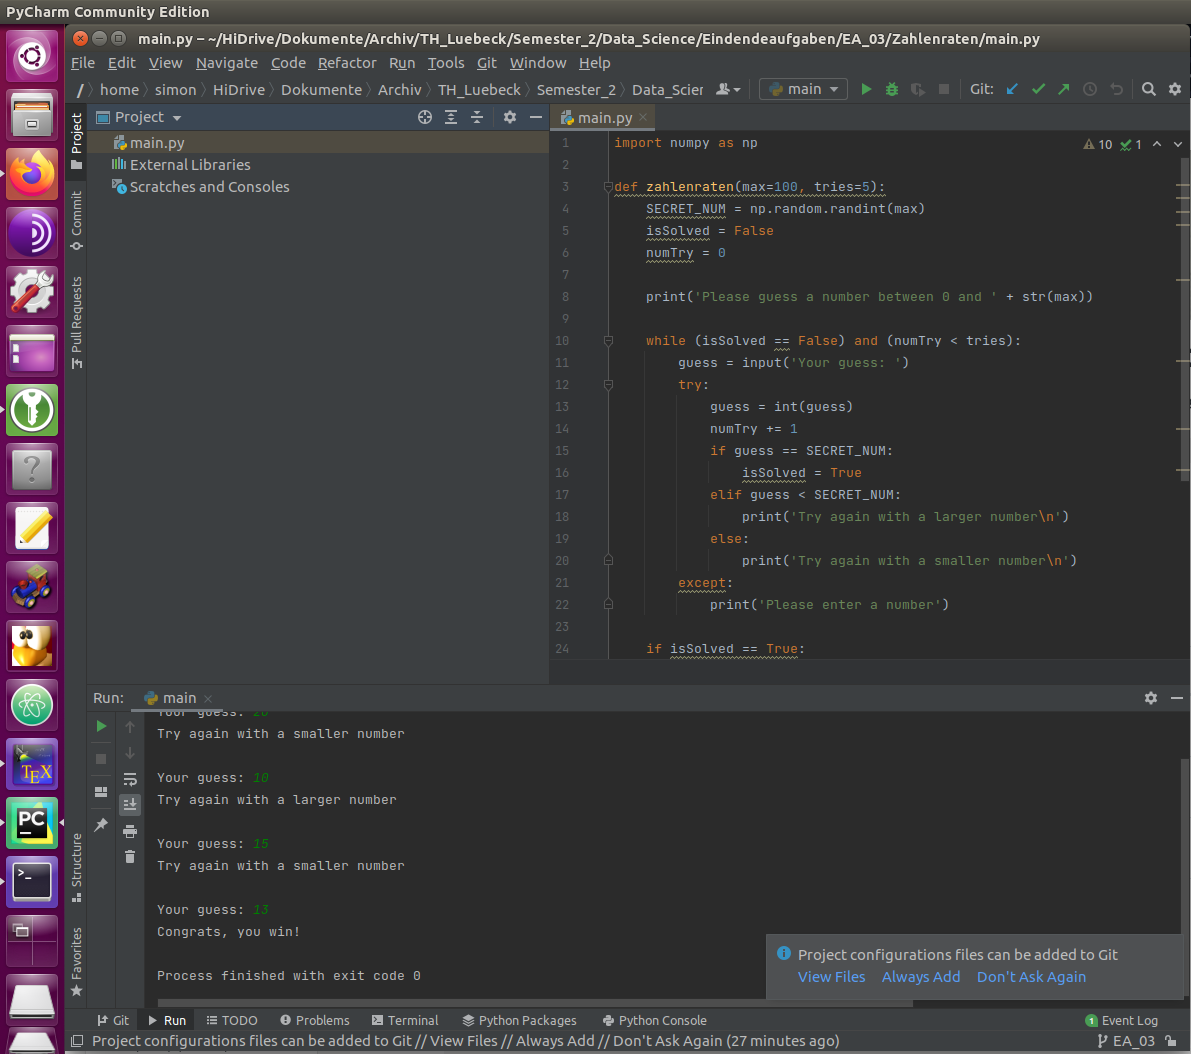
\includegraphics[width=1.0\linewidth]{images/PyCharm}
	\caption[PyCharm]{PyCharm installiert und konfiguriert}
	\label{fig:pycharm}
\end{figure}


\section{Dive into Python}
\textit{A2: Code a little game in Python as Tic Tac Toe, Hangman, Word Guessing / Hangman, Othello, etc. Note that there is no fancy graphics required! Console apps are ok!}

Kleines Zahlenraten in Python:

\lstinputlisting[language=Python, frame=single, tabsize=2, basicstyle=\footnotesize, showstringspaces=false]{Zahlenraten/main.py}


\section{NumPy}
\textit{A3: If you have not done so already, really work through the Quickstart Tutorial from NumPy \footnote{https://numpy.org/doc/stable/user/quickstart.html}}

\lstinputlisting[language=Python, frame=single, tabsize=2, basicstyle=\footnotesize, showstringspaces=false]{Zahlenraten/numpy_quickstart.py}

\section{101 NumPy}
\textit{If you have not done so already, really work through ALL the 101 NumPy exercises\footnote{https://www.machinelearningplus.com/python/101-numpy-exercises-python}. A great way to start from scratch!}

Im Folgenden einige Beisiele:

\lstinputlisting[language=Python, frame=single, tabsize=2, basicstyle=\footnotesize, showstringspaces=false]{Zahlenraten/101.py}

\section{Handson Notebook}
\textit{A5: This is also a wonderful introduction via a notebook \footnote{https://github.com/ageron/handson-ml/blob/master/tools\_numpy.ipynb}}

\section{Pandas}
\textit{A6: If you have not done so already, really work through the 10 min Tutorial from Pandas\footnote{https://pandas.pydata.org/pandas-docs/stable/10min.html}}

\section{SciPy}
\textit{A7: Now work through the tutorials given in the second section here:\footnote{https://docs.scipy.org/doc/scipy/reference/}. Much of the math is hard here but if something looks understandable to you (as basic distribution handling, etc.), then play with it.}
\end{document}
